\documentclass[10pt]{beamer}
\usepackage[utf8]{inputenc} %Allow use of special character
\usepackage{textgreek}
\usepackage{textcomp}

\usetheme{metropolis}
\usepackage{appendixnumberbeamer}
\usepackage[italian]{babel} %Traduce le sezioni in italiano

\usepackage{booktabs}
\usepackage[scale=2]{ccicons}

\usepackage{pgfplots}
\usepgfplotslibrary{dateplot}

%for tables
\usepackage{multirow} %Allows the use of \multirow
\usepackage{array} %For fixed dimension in column
\newcolumntype{K}[1]{>{\centering\arraybackslash}m{#1}} %centred text in fixed width columns

\usepackage[style=chem-rsc, backend=biber, useauthor=false]{biblatex}
\AtEveryCitekey{\ifuseauthor{}{\clearname{author}}}
\AtEveryBibitem{\ifuseauthor{}{\clearname{author}}}
\addbibresource{bibliografia.bib}%Resources for the bibliography

%Package for images ang handling of molecules numbering
\usepackage{graphicx, auto-pst-pdf, chemnum}
\usepackage{float} %Images positioning
\setchemnum{replace-style={\tiny}} %Set the dimension of the replaced number
\graphicspath{{images/}} %Set the directory for images to ./images/nomeimmagine
\usepackage{chemscheme} %Add scheme floating type
\usepackage{mhchem}	%For \ce comand

\usepackage{xcolor}

\def\hnmr{$^1$H-NMR \space}
\def\cnmr{$^{13}$C-NMR \space}
\def\pnmr{$^{31}$P-NMR \space}

\definecolor{red}{HTML}{FF3333}
\definecolor{blue}{HTML}{3333FF}

\usepackage{xspace}

\title{$\alpha$-amminazioni asimmetriche con esteri azodicarbossilici}
\subtitle{Seminario di Tecniche Chimiche Avanzate}
\date{\today}
\author{Mattia Bondanza}
\institute{Università di Pisa}
\titlegraphic{\hfill\includegraphics[height=1.5cm]{cherubino_black.eps}}

\begin{document}

\maketitle

\begin{frame}[fragile]{{\textalpha}-amminazioni}

  Una {\textalpha}-amminazione è una reazione che introduce un gruppo amminico in posizione {\textalpha} ad un \alert{carbonile}.\\
  Danno accesso a {\textalpha}-ammino carbonili come, ad esempio \alert{{\textalpha}-amminoacidi non naturali} o molti composti \alert{biologicamente attivi}. 

  \begin{figure}[H]  	
  	\centering
  	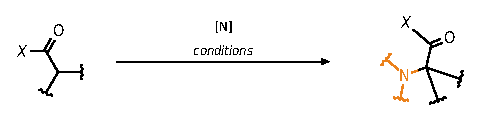
\includegraphics[scale=0.7]{P_general_amination.eps}
  \end{figure}  

\end{frame}

\begin{frame}[fragile]{{\textalpha}-amminazioni}

Sia la maggior parte dei composti all'azoto che il C-{\textalpha} a un gruppo carbonilico hanno caratteri marcatamente nucleofilici.\\
Per ottenere una reazione bisogna quindi:
\begin{enumerate}[(a)]
	\item utilizzare composti \textcolor{red}{elettrofili} all'azoto
	\begin{figure}[H]  	
		\centering
		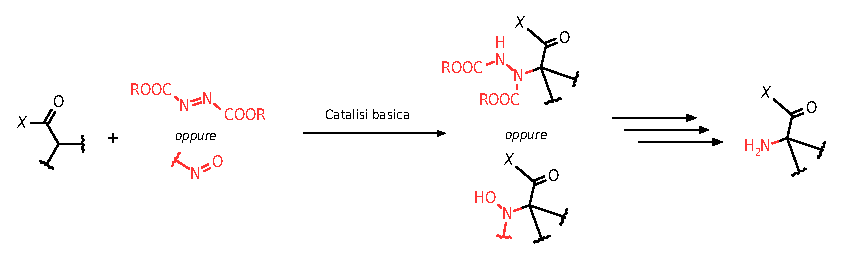
\includegraphics[scale=0.7]{P_electrophile_amination.eps}
	\end{figure}  
	\item utilizzare una miscela di un \textcolor{blue}{nucleofilo} all'azoto e di un ossidante  \footfullcite{delaTorreReversingPolarityCarbonyl2017}
	\begin{figure}[H]  	
		\centering
		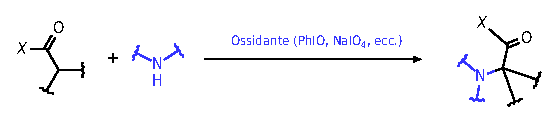
\includegraphics[scale=0.7]{P_nucleophile_amination.eps}
	\end{figure}  
\end{enumerate} 
\end{frame}

\begin{frame}[fragile]{{\textalpha}-amminazioni}

L'uso di reagenti \textcolor{red}{elettrofilici} è stato \alert{ampiamente studiato}, applicato a molti substrati ma necessita di \alert{elaborazioni successive} per rivelare la funzionalità amminica introdotta; i più comuni reattivi elettrofili sono gli azodicarbossilati, le idrossilammine e le solfonilazidi.\\\vspace{3mm}
L'uso di reagenti \textcolor{blue}{nucleofilici} è un campo emergente, è applicato principalmente a \alert{carbonili reattivi} (aldeidi, chetoni, {\textalpha},{\textbeta}-dicarbonili, ecc.) ed è richiesto l'impiego di un equivalente \alert{stechiometrico di ossidante}.\\
\end{frame}

\begin{frame}[fragile]{{\textalpha}-amminazioni con azodicarbossilati}
I reagenti elettrofili all'azoto più diffusi sono gli \alert{azodicarbossilati}:
  \begin{figure}[H]  	
	\centering
	
\includegraphics[scale=0.7]{P_azodicarboxylate.eps}
\end{figure}  

\begin{itemize}
	\item[--] in molti casi sono commercialmente disponibili,
	\item[--] sono elettrofili energici e reagiscono efficacemente con molti substrati,
	\item[--] \alert{l'elaborazione successiva è fortemente dipendente azodicarbossilato utilizzato},
	\item[--] l'introduzione di unità amminiche secondarie o terziarie richiede diversi step sintetici.
\end{itemize}

\end{frame}

\begin{frame}[fragile]{Elaborazione dei prodotti di {\textalpha}A degli azodicarbossilati}
\begin{figure}[H]  	
	\centering
	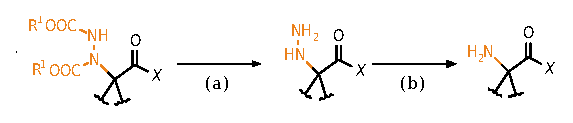
\includegraphics[scale=0.7]{P_genericelaboration.eps}
\end{figure}  
Per rivelare la funzionalità amminica dai prodotti di amminazione derivanti dagli azodicarbossilati sono necessari due passaggi:
\begin{enumerate}[(i)]
	\item la rimozione dei gruppi protettori sull'unità idrazinica,
	\item la fissione del legame \ce{NH-NH2}.
\end{enumerate}
\end{frame}

\begin{frame}[fragile]{Elaborazione dei prodotti di {\textalpha}A degli azodicarbossilati}
\begin{figure}[H]  	
	\centering
	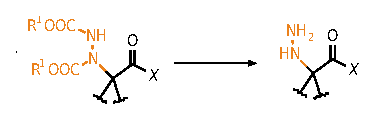
\includegraphics[scale=0.7]{P_elaboration1.eps}
\end{figure}  
	La rimozione dei gruppi protettori può essere effettuata in \alert{condizioni blande se R$^1$ = $^t$Bu}; richiede invece condizioni molto drastiche se R$^1$ = $^i$Pr, Et; quando R$^1$ = Bn è possibile applicare protocolli idrogenolitici.
	\begin{table}[H]
		\begin{tabular}{K{1cm} K{4cm} K{4cm}}
			COOR$^1$ & Condizioni di sblocco & Problemi\\ 
			\hline \\
			COOEt & KOH 2.5 M in $^i$PrOH, riflusso, 4 h  & basse rese, retro-amminazione\\	
			COO$^i$Pr & conc. HCl, reflux, 23 h & degradazione del substrato\\		
			\alert{Boc} & \alert{HCl o TFA in solvente organico RT, 1 -- 3 h} & -\\	
			Cbz & Pd/C (10\%), H$_2$ in MeOH, RT & (retro-amminazione)\\
			\hline
		\end{tabular}
	\end{table}

\end{frame}

\begin{frame}[fragile]{Elaborazione dei prodotti di {\textalpha}A degli azodicarbossilati}
\begin{figure}[H]  	
	\centering
	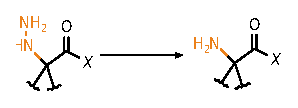
\includegraphics[scale=0.7]{P_elaboration2.eps}
\end{figure}  
La fissione del legame \ce{NH-NH2} richiede normalmente \alert{condizioni idrogenolitiche}. I catalizzatori più usati sono stati il Ni/Raney, Pd/C e Rh/C\footfullcite{ZhouOrganocatalyticAsymmetricaAmination2011}. Alcuni autori sostengono che quando non si utilizzi Rh/C si registri una estensiva formazione del prodotto deamminato (fissione del legame \ce{C-NH})\footfullcite{ShibasakiCatalyticAsymmetricAmination2012}.\\
In ogni caso sulla molecola non possono essere presenti gruppi sensibili all'idrogenazione catalitica (\ce{-C#N}, \ce{C=C}, \ce{C#C}, \ldots)

\end{frame}

\begin{frame}[fragile]{{\textalpha}-amminazioni asimmetriche}

\begin{figure}[H]  	
	\centering
	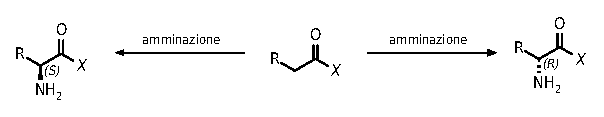
\includegraphics[scale=0.7]{P_enantioelective_amination.eps}
\end{figure}  

Quando la reazione è condotta su un substrato la avente un \alert{C$_{\alpha}$ prochirale}, si possono formare due prodotti che si differenziano per la configurazione assoluta del nuovo centro stereogenico, ovvero sono \alert{enantiomeri o epimeri}.\\
Lo sviluppo di metodi per controllare il \alert{decorso stereochimico} di questo tipo di reazioni è importante in quanto questi composti sono studiati per applicazioni in ambito biologico.
\end{frame}

\begin{frame}[fragile]{{\textalpha}-amminazioni diasereoselettive}
I primi lavori nel settore hanno riguardato \alert{amminazioni diastereoselettive}.\\
Evans \textit{et al.} propongono ad esempio l'amminazione di un'ammide utilizando un ossazolidinone chirale come gruppo protettore \footfullcite{Evansasymmetricsynthesisaamino1988}.\\ 
\begin{figure}[H] 
	\replacecmpd{evans1}
	\replacecmpd{evans2}
	\replacecmpd{dtbad} 	
	\centering
	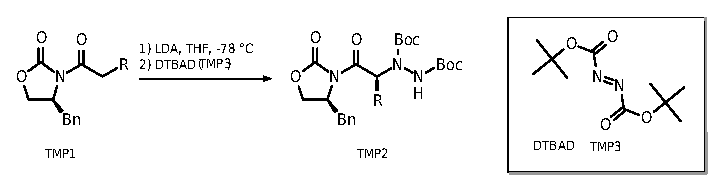
\includegraphics[scale=0.7]{P_diastereoevans.eps}
\end{figure}  
Questo approccio è svantaggioso in quanto richiede l'uso di una quantità \alert{stechiometrica} sia di base che di \alert{ausiliario chirale}.

\end{frame}

\begin{frame}[fragile]{{\textalpha}-amminazioni enantioselettive}
Per superare i difetti degli approcci diastereoselettivi Evans \textit{et al.} propongono una \alert{versione enantioselettiva} della reazione.\\
La funzionalità carbossilica viene protetta con un ossazolidinone non chirale e viene introdotto \alert{un sistema catalitico chirale}, basato sul complesso di magnesio \cmpd{evans_cat} che trasferisce chiralità al prodotto \footfullcite{EvansChiralmagnesiumbis1997}.

La reazione risulta ancora limitata nello scopo e necessita di un sistema di protezione della funzionalità carbossilica per funzionare.
\end{frame}

\begin{frame}[fragile]{{\textalpha}-amminazioni enantioselettive}
I gruppi di B. List e K. J\o rgensen svilupparono in maniera contemporanea un nuovo protocollo di \textalpha-amminazione asimmetrica per \alert{aldeidi, chetoni} e altri carbonili facilmente enolizzabili basata sull'uso della \alert{(L)-prolina} (\cmpd{proline}) come organocatalizzatore chirale \footfullcite{ListDirectCatalyticAsymmetric2002}$^,$ \footfullcite{BogevigDirectOrganoCatalyticAsymmetricaAmination2002}.
\begin{figure}[H] 
	\replacecmpd{listproduct}
	\replacecmpd{proline} 	
	\replacecmpd{dtbad}
	\centering
	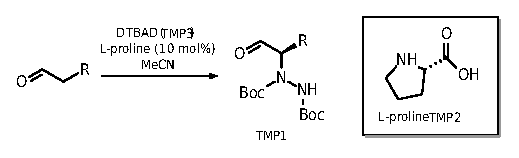
\includegraphics[scale=0.7]{P_listorganoaaa.eps}
\end{figure}  
\end{frame}

\begin{frame}[fragile]{{\textalpha}-amminazioni enantioselettive}
La reazione di {\textalpha}-amminazione asimmetrica basata sulla prolina è stata studiata intensamente e si è proposto un probabile \alert{stato di transizione} (\cmpd{mfzt}) confermato sia da evidenze sperimentali\footfullcite{HeinEnamineCarboxylatesStereodetermining2011} che da calcoli DFT\footfullcite{Furevisitprolinecatalyzedamination2015}.
\begin{figure}[H] 
	\replacecmpd{mfzt}
	\centering
	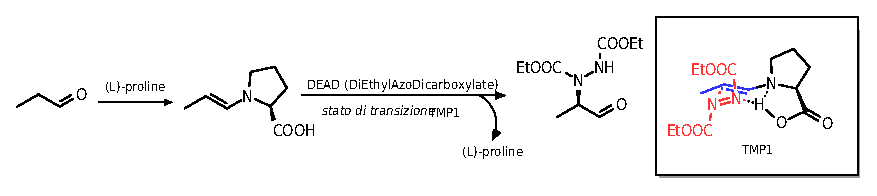
\includegraphics[scale=0.7]{P_mfzt.eps}
\end{figure}  
Lo stato di transizione proposto implica che la reazione proceda per la formazione dell'\alert{enammina del composto carbonilico} su cui attacca l'elettrofilo.
\end{frame}

\begin{frame}[fragile]{{\textalpha}-amminazioni enantioselettive}
Le catalisi via formazione dell'enammina è intrinsecamente \alert{limitata a substrati facilmente enolizzabili}.\\
Sono stati proposti metodi basati sulla semplice \alert{catalisi basica}, in particolare sull'utilizzo di \alert{derivati degli alcaloidi di cincona}.\\
Uno dei primi esempi è riportato da J\o rgensen \textit{et al.}:
\begin{figure}[H] 
	\replacecmpd{dtbad}
	\centering
	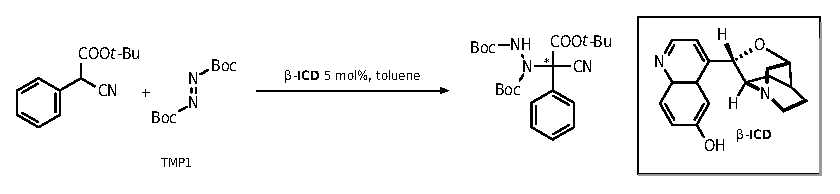
\includegraphics[scale=0.7]{P_firstcinchona.eps}
\end{figure}  

\end{frame}

\begin{frame}[fragile]{{\textalpha}-amminazioni enantioselettive}
In questo caso la chiralità è trasferita dal catalizzatore al prodotto attraverso la \alert{formazione all'equilibrio di un enolato} avente come controione il catalizzatore protonato \footfullcite{BuiExpandingScopeCinchona2009}.
\begin{figure}[H] 
	\replacecmpd{dtbad}
	\centering
	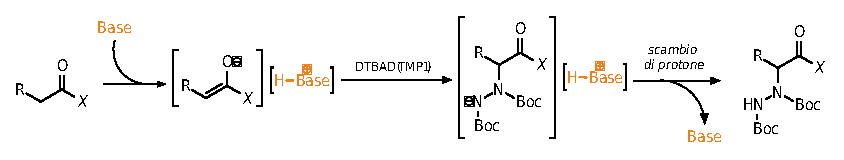
\includegraphics[scale=0.7]{P_basecat_amination.eps}
\end{figure}  
In queste condizioni è possibile amminare anche \alert{composti carbonilici poco reattivi}.\\
Lo specifico meccanismo di induzione asimmetrica dipende dalla base catalitica usata; i solventi hanno una forte influenza.

\end{frame}

\begin{frame}[fragile]{{\textalpha}-amminazioni enantioselettive sui 2-ossindoli}
Dei substrati particolarmente interessanti per queste reazioni sono i 2-ossindoli; pur essendo formalmente dei \textit{lattami} hanno un'\alert{acidità al C$_{\alpha}$ notevolmente superiore a normali ammidi}\footfullcite{BordwellHeterocyclicaromaticanions1991}.\\
\begin{figure}[H] 
	\centering
	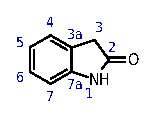
\includegraphics[scale=0.7]{P_oxindolering.eps}
\end{figure} 
Molti 3-ammino-2-ossindoli sono composti con \alert{interesse biologico}.
\begin{figure}[H] 
	\centering
	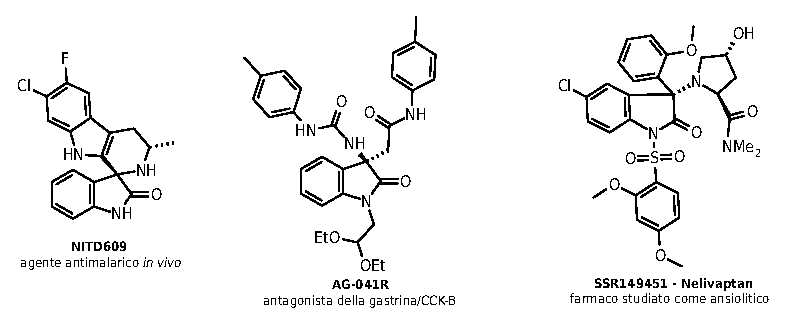
\includegraphics[scale=0.7]{P_oxindoledrugs.eps}
\end{figure} 
\end{frame}

\begin{frame}[fragile]{{\textalpha}-amminazioni enantioselettive sui 2-ossindoli}
Sono stati sviluppati \alert{diversi protocolli} per l'amminazione di questi composti che si differenziano per:
\begin{itemize}
	\item[--] l'azodicarbossilato usato,
	\item[--] il sistema catalitico usato,
	\item[--] il livello di sostituzione tollerato alle posizioni 1 e 3 del sistema 2-ossindolico,
	\item[--] il grado di induzione asimmetrica raggiunto dalla reazione.	
\end{itemize}
\end{frame}

\begin{frame}[fragile]{{\textalpha}-amminazioni enantioselettive sui 2-ossindoli}
Il primi protocolli proposti sono quelli di Chen \textit{et al.}\footfullcite{ChenHighlyEnantioselectiveOrganocatalytic2009} e  Zhou \textit{et al.}\footfullcite{QianAsymmetricconstructionquaternary2009} in cui sono usati i \alert{derivati dimerici degli alcoloidi di cincona} \textbf{\ce{(DHQD)2PHAL}} e \textbf{\ce{(DHQD)2PYR}}.
\begin{figure}[H] 
	\replacecmpd{diad}
	\centering
	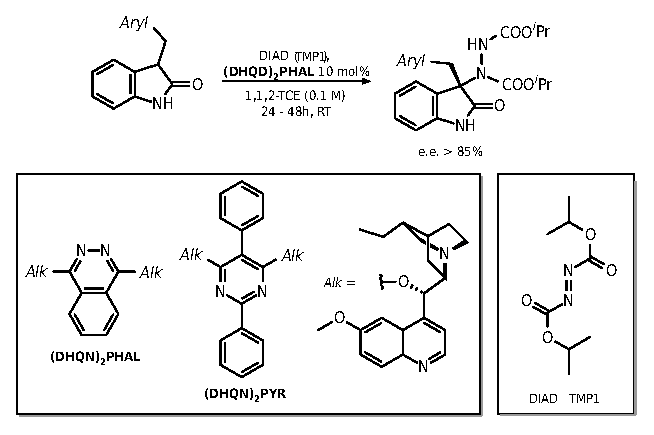
\includegraphics[scale=0.7]{P_chenoaaa.eps}
\end{figure} 
\end{frame}

\begin{frame}[fragile]{{\textalpha}-amminazioni enantioselettive sui 2-ossindoli}
Un protocollo successivo proposto da Barbas III \textit{et al.} \footfullcite{BuiHighlyEnantioselectiveOrganocatalytic2010} propone l'utilizzo di un sistema catalitico non commerciale (\cmpd{barbascat}) per amminare \alert{3-aril-2-ossindoli}.
\begin{figure}[H] 
	\replacecmpd{dtbad}
	\replacecmpd{barbascat}
	\centering
	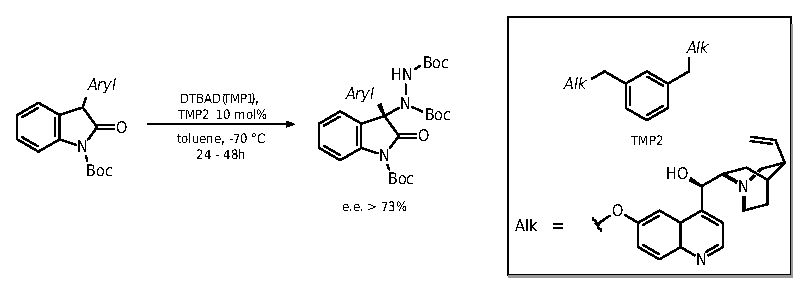
\includegraphics[scale=0.7]{P_barbas2oaaa.eps}
\end{figure} 
\end{frame}

\begin{frame}[fragile]{{\textalpha}-amminazioni enantioselettive sui 2-ossindoli}
Il protocollo che ad oggi ha si presenta come il più generale è quello proposto da Shibasaki \textit{et al.} \footfullcite{ShibasakiCatalyticAsymmetricAmination2012}.\\
Questo protocollo utilizza però un \alert{sistema catalitico basato sul nikel}
\begin{figure}[H] 
	\replacecmpd{shibasakicat}
	\replacecmpd{dtbad}
	\centering
	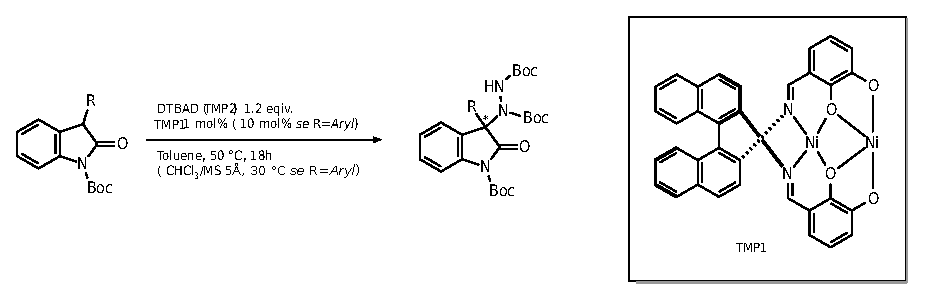
\includegraphics[scale=0.7]{P_shibasakioaaa.eps}
\end{figure} 
La reazione è stata utilizzata per effettuare una sintesi formale del composto biologicamente attivo \alert{AG-041R}.
\end{frame}


\begin{frame}[standout]
  Domande?
\end{frame}

\begin{frame}{Source}

\begin{center}
	I sorgenti di questa presentazione sono liberamente scaricabili da:
\end{center}

\begin{center}\url{github.com/Biondilbiondo/seminarioLTCA}\end{center}

\begin{center}\ccbysa\end{center}

\end{frame}

\appendix


\end{document}
